%% This is file `elsarticle-template-2-harv.tex',
%%
%% Copyright 2009 Elsevier Ltd
%%
%% This file is part of the 'Elsarticle Bundle'.
%% ---------------------------------------------
%%
%% It may be distributed under the conditions of the LaTeX Project Public
%% License, either version 1.2 of this license or (at your option) any
%% later version.  The latest version of this license is in
%%    http://www.latex-project.org/lppl.txt
%% and version 1.2 or later is part of all distributions of LaTeX
%% version 1999/12/01 or later.
%%
%% The list of all files belonging to the 'Elsarticle Bundle' is
%% given in the file `manifest.txt'.
%%
%% Template article for Elsevier's document class `elsarticle'
%% with harvard style bibliographic references
%%
%% $Id: elsarticle-template-2-harv.tex 155 2009-10-08 05:35:05Z rishi $
%% $URL: http://lenova.river-valley.com/svn/elsbst/trunk/elsarticle-template-2-harv.tex $
%%
\documentclass[preprint,authoryear,12pt]{elsarticle}

%% Use the option review to obtain double line spacing
%%\documentclass[authoryear,preprint,review,12pt]{elsarticle}

%% Use the options 1p,twocolumn; 3p; 3p,twocolumn; 5p; or 5p,twocolumn
%% for a journal layout:
%% \documentclass[final,authoryear,1p,times]{elsarticle}
%% \documentclass[final,authoryear,1p,times,twocolumn]{elsarticle}
%% \documentclass[final,authoryear,3p,times]{elsarticle}
%% \documentclass[final,authoryear,3p,times,twocolumn]{elsarticle}
%% \documentclass[final,authoryear,5p,times]{elsarticle}
%% \documentclass[final,authoryear,5p,times,twocolumn]{elsarticle}

%% if you use PostScript figures in your article
%% use the graphics package for simple commands
%%\usepackage{graphics}
%% or use the graphicx package for more complicated commands
 \usepackage{graphicx}
 \graphicspath{ {../img/au/} {../img/us/}{../img/in/}}
%% or use the epsfig package if you prefer to use the old commands
%% \usepackage{epsfig}

%% The amssymb package provides various useful mathematical symbols
\usepackage{amssymb}
%% The amsthm package provides extended theorem environments
\usepackage{amsthm}

%% The lineno packages adds line numbers. Start line numbering with
%% \begin{linenumbers}, end it with \end{linenumbers}. Or switch it on
%% for the whole article with \linenumbers after \end{frontmatter}.
%% \usepackage{lineno}

%% natbib.sty is loaded by default. However, natbib options can be
%% provided with \biboptions{...} command. Following options are
%% valid:

%%   round  -  round parentheses are used (default)
%%   square -  square brackets are used   [option]
%%   curly  -  curly braces are used      {option}
%%   angle  -  angle brackets are used    <option>
%%   semicolon  -  multiple citations separated by semi-colon (default)
%%   colon  - same as semicolon, an earlier confusion
%%   comma  -  separated by comma
%%   authoryear - selects author-year citations (default)
%%   numbers-  selects numerical citations
%%   super  -  numerical citations as superscripts
%%   sort   -  sorts multiple citations according to order in ref. list
%%   sort&compress   -  like sort, but also compresses numerical citations
%%   compress - compresses without sorting
%%   longnamesfirst  -  makes first citation full author list
%%
\biboptions{square,comma}

% \biboptions{}

\journal{ }

\begin{document}
	
	\begin{frontmatter}
		
		%% Title, authors and addresses
		
		%% use the tnoteref command within \title for footnotes;
		%% use the tnotetext command for the associated footnote;
		%% use the fnref command within \author or \address for footnotes;
		%% use the fntext command for the associated footnote;
		%% use the corref command within \author for corresponding author footnotes;
		%% use the cortext command for the associated footnote;
		%% use the ead command for the email address,
		%% and the form \ead[url] for the home page:
		%%
		%% \title{Title\tnoteref{label1}}
		%% \tnotetext[label1]{}
		%% \author{Name\corref{cor1}\fnref{label2}}
		%% \ead{email address}
		%% \ead[url]{home page}
		%% \fntext[label2]{}
		%% \cortext[cor1]{}
		%% \address{Address\fnref{label3}}
		%% \fntext[label3]{}
		
		\title{A Study on The Effectiveness of Lock-down Measures to Control The Spread of COVID-19}
		
		%% use optional labels to link authors explicitly to addresses:
		%% \author[label1,label2]{<author name>}
		%% \address[label1]{<address>}
		%% \address[label2]{<address>}
		
		\author[a1]{Subhas Kumar Ghosh\corref{cor1}}
		\ead{subhas.ghosh@cba.com.au}
		\author[a2]{Sai Shanmukha Narumanchi}
		\ead{sai@cs.siu.edu}
		\author[a2]{Koushik Sinha}
		\ead{koushik.sinha@@cs.siu.edu}
		
		\cortext[cor1]{Corresponding author}
		\address[a1]{Commonwealth Bank of Australia, Sydney, New South Wales, 2000, Australia}
		\address[a2]{Department of Computer Science, Southern Illinois University, Carbondale, IL 62901, USA.}
		
		\begin{abstract}
			%% Text of abstract
			
		\end{abstract}
		
		\begin{keyword}
			%% keywords here, in the form: keyword \sep keyword
			COVID-19 \sep Lock down \sep Mathematical modeling \sep Epidemic \sep Economic Impact
			
			%% MSC codes here, in the form: \MSC code \sep code
			%% or \MSC[2008] code \sep code (2000 is the default)
			
		\end{keyword}
		
	\end{frontmatter}
	
	% \linenumbers
	
	%% main text
	\section{Introduction}
	\label{SEC1}
	In December 2019, a zoonotic coronavirus, similar to SARS coronavirus and MERS coronavirus outbreak occurred in Wuhan, China \cite{taaa021}.  Afterwards, the virus has been named as Severe Acute Respiratory Syndrome Coronavirus 2 (SARS-CoV-2), and disease caused by the virus has been named coronavirus disease 2019 (COVID-19). Since then the ongoing pandemic has infected more 6 million people and has caused 300 thousand deaths worldwide .
	
	Initial estimate of $R_0$, and mortality rate. 
	
	Non availability of treatment paradigm and any defense mechanism like vaccination.
	 
	Treatment requiring ventilation for long time - requirement was to reduce pressure on healthcare system - SIR modeling forecast 
	
	Option available for policymakers was to issue wide scale lock-down / home stay orders, social distancing measures, closing down non-essential 
	
	Led to - what are the impacts and losses
	
	Motivate the requirements for analyzing effectiveness of lock-down.   What were the benefits? Reducing burden on healthcare system, saving loss of life, and reducing $R_0$ by breaking transmission chain. 
	
	How can we measure these benefits and compare with the economic losses?
	
	\subsection{Our contribution}
	Defining how to measure these benefits.
	
	Tools for measuring them.
	
	
	Difficulty in assessing: different level of compliance, different cultural practices - hidden variables
	
	\subsection{Related Works}
	Other modeling approaches. SIR-F, DCM, Agent, Hybrid - not post fact A/B testing tools.
	
	\subsection{Tools}
	
	$m-RSC$ \cite{ap08746, JMLR18}, Trend analysis, 
	
	
	
	\section{The setup}
    \label{SEC2}
	Data - Data Source - Dims [infected, fatal, recovered, No of tests] 
	
	
	
	\section{Results}
	\label{SEC3}
	
	India - 4 stages of lock-down - effect of each stages - results on prediction by Synthetic control
\begin{figure}[ht]
	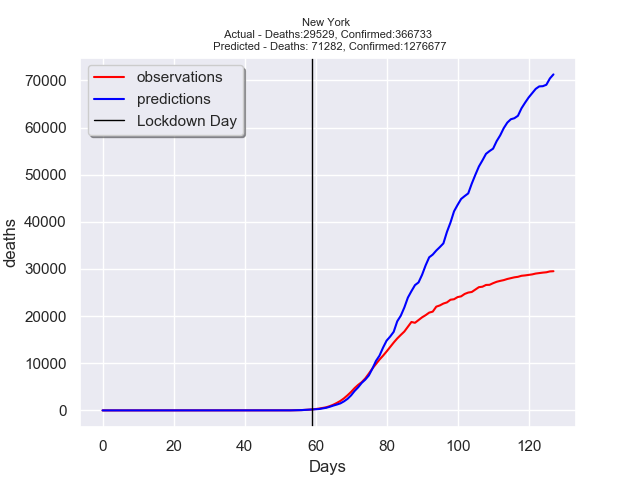
\includegraphics[width=0.7\textwidth]{New York}
\end{figure}

	Singapore - recurrence - change in projection on those dates
	
	US - compare prediction models data vs. Synthetic control projection vs actual by state by start and end of lock-down dates (what are the control group in each cases)
	
	AU NZ South K
	
	Sweden
	
	Measured results. 
	
	\section{Discussion}
	\label{SEC4}
	
	
	\section{Concluding Remarks}
	\label{SEC5}
	%% References
	
	\bibliographystyle{elsarticle-num}
	\bibliography{lockdown.bib}	
\end{document}

%%
%% End of file `elsarticle-template-2-harv.tex'.
